%% ----------------------------------------------------------------
%% Article.tex
%% ---------------------------------------------------------------- 
\documentclass{ecsarticle}     % Use the Article Style
\graphicspath{{Figures/}}   % Location of your graphics files
\usepackage{natbib}            % Use Natbib style for the refs.
\hypersetup{colorlinks=false}   % Set to false for black/white printing
\input{Definitions}            % Include your abbreviations

\usepackage[nodayofweek]{datetime}
\usepackage{listings}
\usepackage{color}

\usepackage{graphicx}



%% ----------------------------------------------------------------
\begin{document}
%TC:ignore
\frontmatter
\title      {COMP6036: Advanced Machine Learning\\
            An investigation into DBSCAN}
      
\addresses  {\deptname\\\univname}
\authors                 {\href{mailto:ajr2g10@ecs.soton.ac.uk}{Ashley J. Robinson}\\\href{mailto:ajr2g10@ecs.soton.ac.uk}{ajr2g10@ecs.soton.ac.uk}}

\date       {\today}
\subject    {}
\keywords   {}
\maketitle
%% ----------------------------------------------------------------


\begin{abstract}
The paper chosen for the research report is entitled \textbf{A density-based algorithm for discovering clusters in large spatial databases with noise} which introduces the algorithm DBSCAN.
DBSCAN is used for clustering sparse spatial databases using data point density.
The algorithm performs well at this but has some shortcomings when applied to tasks which hold clusters of different densities.
Only one priori, cluster density, is required but the algorithm is very sensitive to this and can be difficult to tune in high dimensional space.
DBSCAN is compared against other common cluster implementations using a machine learning toolkit for Python before more recent extensions are considered.
\end{abstract}

%TC:endignore
\mainmatter


\section{Motivation for Algorithm}

DBSCAN (Density-Based Spatial Clustering of Applications with Noise) is an unsupervised application of machine learning introduced by~\cite{ester96dbscan}.
Intended to address Spatial Database Systems (SDBS) which can be produced from naturally occurring geometric and geographical data or engineering applications such a layout for integrated circuit design~\citep{guting94sdbs}.
It has three main objectives.
To minimise the required domain knowledge needed to set input parameters, have the capability to discover clusters of arbitrary shapes and to perform well on large spatial databases.

At the time of creation the algorithms was compared to a recent development called CALARANS~\citep{ng94clarans} which is an extension of CLARA (Clustering LARge Applications)~\citep{kaufman90clara}.
Both algorithms are intended for use on large databases but CLARANS uses random noise to improve performance.
Apart from traditional clustering algorithms where first principles are introduced, such a K-means, DBSCAN was a breakthrough in terms of a density approach to datasets.

\section{Technical Explanation}

DBSCAN uses cluster density to classify data.
It is intuitive to build a community of data points by attempting to draw a path of connectivity between points.
This leads to the first input parameter to the algorithm, $\epsilon$, which is a threshold for the distance that DBSCAN is permitted to move yet remain in the same cluster.
Equation~\eqref{eqn:dist}, adapted from~\cite{ester96dbscan}, is the basic function used to determine membership by thresholding; euclidean distance is used in this case but the measure of distance can be replaced with a Manhattan norm to scale down computational overheads therefore favouring large datasets~\citep{krause86taxicab}.
Only two input patterns are compared at once and all belong to the set of training data, $\textbf{x}$, containing $n$ input patterns.

\begin{equation}
	N(\textbf{p},\textbf{q},\epsilon) = \left\{
		\begin{array}{l}
    		1,\: ||\textbf{p} - \textbf{q}|| \leq \epsilon\\
    		0,\: ||\textbf{p} - \textbf{q}|| > \epsilon
  		\end{array} \right.
	\:\:where\:\: \textbf{q},\textbf{p} \in \textbf{x}
	\label{eqn:dist}
\end{equation}


This approach is simple for compact clusters but when noise is introduced the algorithm will identify a few points as a whole cluster.
This is possibly down to a badly tuned value for $\epsilon$ but can be negated by introducing a second threshold to set the minimum number of members a cluster can have however this is unnecessary to perform basic DBSCAN clustering.
Equation~\eqref{eqn:member} takes the sum of connected data points attributed to a single point which used for the comparison in Equation~\eqref{eqn:inside}. 
The parameter, $\lambda$, if successfully applied to Equation~\eqref{eqn:inside} decides when to build a cluster around the point.

\begin{equation}
	C(\textbf{x}_i,\textbf{x},\epsilon) =  \sum\limits_{j=1 \atop j\:\neq\:i}^n N(\textbf{x}_i,\textbf{x}_j,\epsilon)	
	\label{eqn:member}
\end{equation}

\begin{equation}
	1 \leq \lambda \leq C(\textbf{p},\epsilon)\:\:where\:\:\lambda \in \mathbb{N}
	\label{eqn:inside}
\end{equation}

A low dimensional representation of the constraints used in DBSCAN is held in Figure~\ref{fig:circles} which contains seven points labelled \textbf{A} to \textbf{H}.
A string of points are density connected in the centre of the diagram, two points on the left and is \textbf{G} is unconnected.
Increasing $\epsilon$ will merge these three possible clusters.
Equation~\eqref{eqn:clusters} describes how possible values of $\lambda$ can change the clustering of Figure~\ref{fig:circles}.


\begin{figure}[ht]
   \centering
    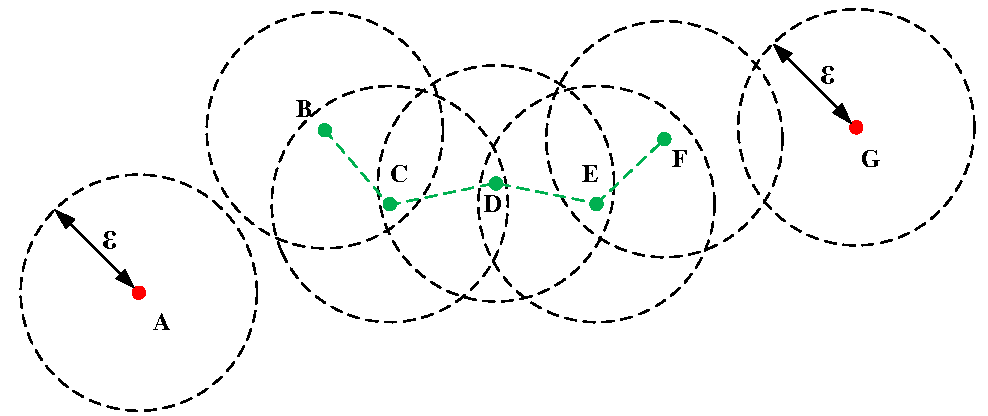
\includegraphics[height = 4cm]{circles.pdf}
   \caption{2D application of DBSCAN.}
   \label{fig:circles}
\end{figure}

\begin{equation}
	\# Clusters = \left\{
		\begin{array}{l}
    		0\:if\; \lambda \geq 6\\
    		1\:if\; \lambda = 5 \\
			2\:if\; 2 \leq \lambda \leq 5 \\
			3\:if\; \lambda = 1\\
  		\end{array} \right.
	\label{eqn:clusters}
\end{equation}




It is clear there is a lot of scope for optimisation in practice.
A list containing all data points at the start of the algorithm can be used to check off points which have been found to belong to a cluster.
This means for an input space containing $\alpha$ clusters that can be perfectly segmented by DBSCAN requires only $\alpha$ calls of Equation~\eqref{eqn:member}.
Formally a set of unclassified vectors, $\textbf{b} \in \textbf{x} $, can be defined and passed to Equation~\eqref{eqn:member} requiring much fewer evaluations. 


\section{Performance}
\label{performance}

The worst case performance of the basic algorithm is determined by the number of end cluster found by DBSCAN compared to the number of input patterns.
If all the input patterns combined with a massive value of $\epsilon$ produce single cluster classification it is possible that $O(n)$ holds; this is based on the number of times Equation~\eqref{eqn:dist} has to be computed.
Equation~\eqref{eqn:order} shows how as the number of clusters increases the algorithm tends towards $O(n^2)$.
The first input pattern requires $n-1$ calls of Equation~\eqref{eqn:dist} regardless but in the worst case is has no reachable neighbours.
The second requires $n-2$ as one pattern has already been identified as solitary yet again has no reachable neighbours.
If this continues so that the last pattern is known to be solitary then Equation~\eqref{eqn:order} shows how this geometric progression places an lower bound on performances.
A well tuned value of $\epsilon$ will allow the algorithm to complete in polynomial time.

\begin{equation}
	\sum\limits_{i=1}^{n-1} i = \frac{n}{2}(n - 1) \approx O(n^2)	
	\label{eqn:order}
\end{equation}


DBSCAN suffers from sensitivity to input parameters and clustering in high dimensional space~\cite{han01survey}.
When attempting to cluster regions of different density it is clear that this is a major problem for the algorithm in certain applications. 
The graphs in Figure~\ref{fig:compare} are different clustering algorithms applied to a shape dataset taken from~\cite{gionis05cluster} which is chosen to empathise some less obvious shortcomings.
Chosen for comparison is K-Means because it is arguably the most well-known clustering algorithm and WARD because of its performance on this dataset when compared against other available algorithms.
Implementations\footnote{Code in Appendix~\ref{code}} were taken from a machine learning toolbox for Python~\citep{scikit13ml}.
The dataset contains seven clusters but in two cases there are \emph{bridges} between the clusters.
On the far right K-Means and WARD correctly divides the data where DBSCAN incorrectly groups both clusters together; shown in Figures~\ref{fig:kmeans},~\ref{fig:ward} and~\ref{fig:dbscan} respectively.
DBSCAN deals well with the remaining data where the other two algorithms fail due to its ability to negate relatively tight clusters.
These sorts of issues are the reason for $\epsilon$ sensitivity. 

\begin{figure}[ht]
   \centering
   \subfigure[K-Means]{
      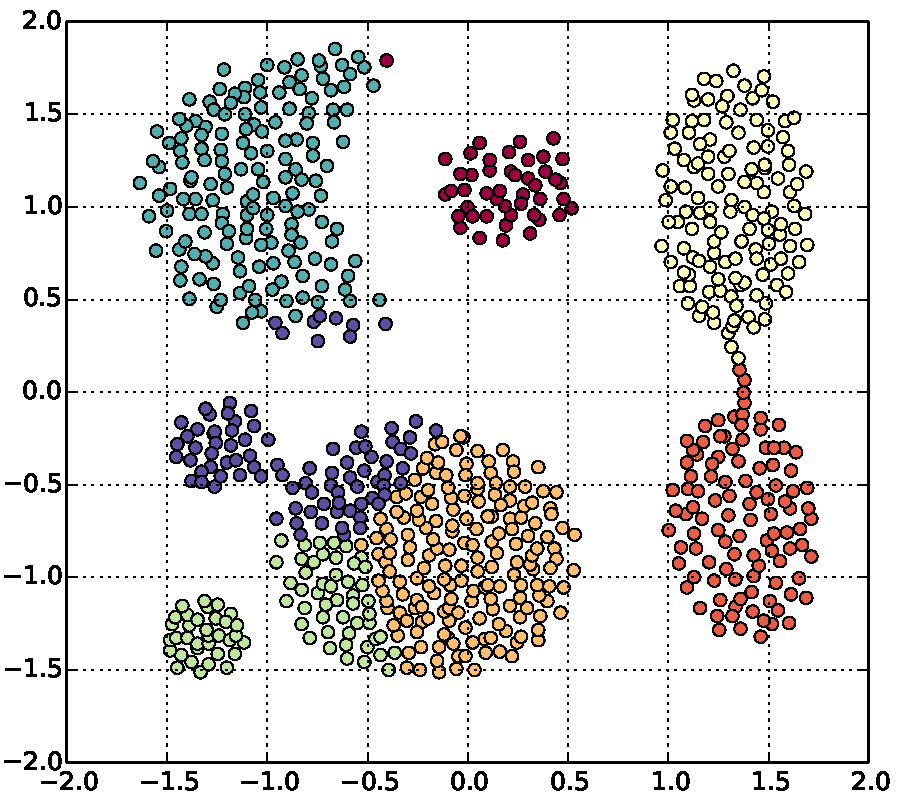
\includegraphics[height = 5cm,width = 5cm]{kmeans.pdf}
      \label{fig:kmeans}
   }
   \subfigure[WARD]{
      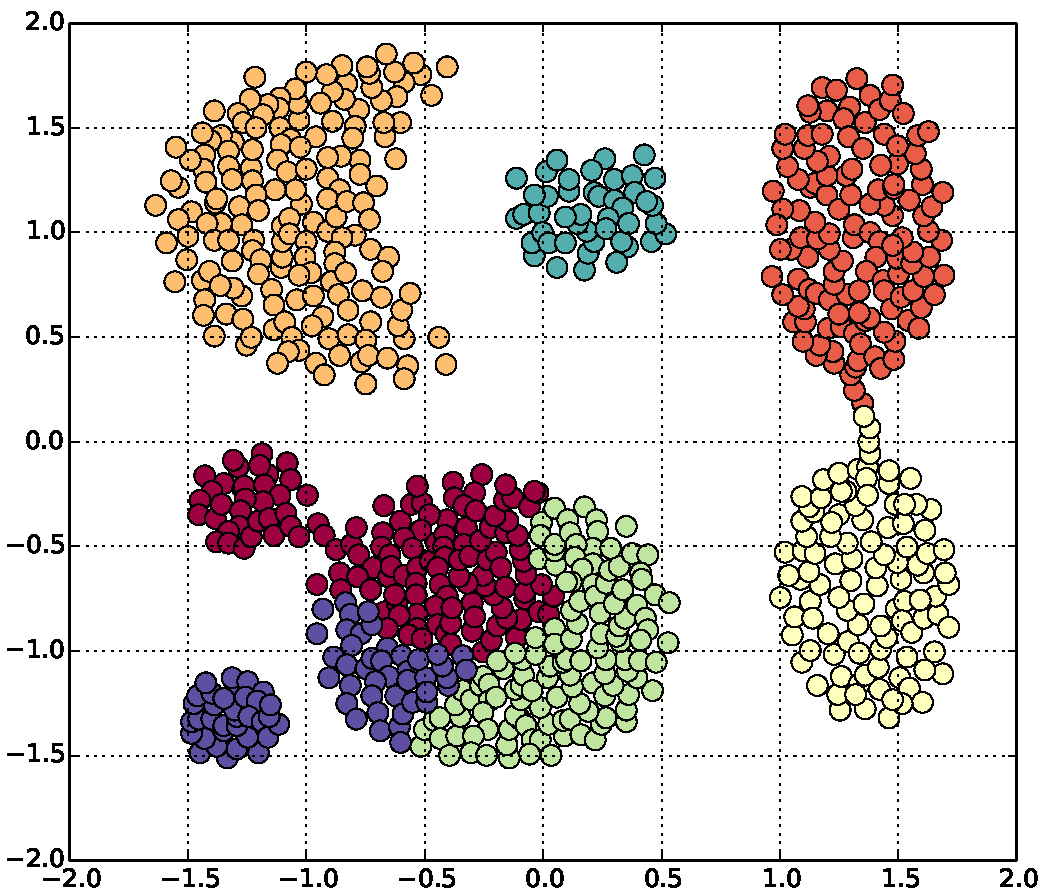
\includegraphics[height = 5cm, width = 5cm]{ward.pdf}
      \label{fig:ward}
   }
   \subfigure[DBSCAN]{
      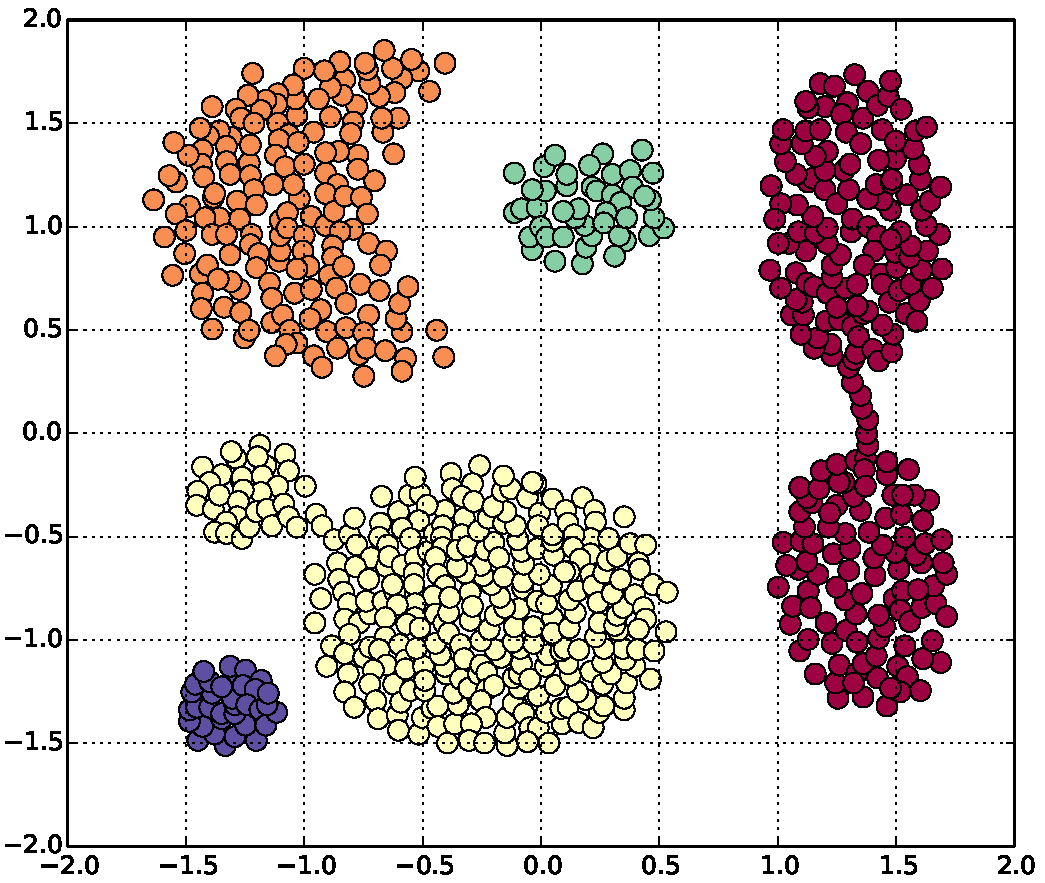
\includegraphics[height = 5cm,width = 5cm]{dbscan.pdf}
      \label{fig:dbscan}
   }
   \caption{A comparison against DBSCAN.}
   \label{fig:compare}
\end{figure}

The algorithm exhibits variation in performance as per the standard bias-variance dilemma.
Figure~\ref{fig:error} shows how the error varies for with $\epsilon$ when applied to data used in Figure~\ref{fig:compare}.
Objectively DBSCAN doesn't perform well on this dataset missing two clusters completely however this is a crafted cornerstone case intended to trap algorithms and is not particularly sparse.

\begin{figure}[ht]
   \centering
    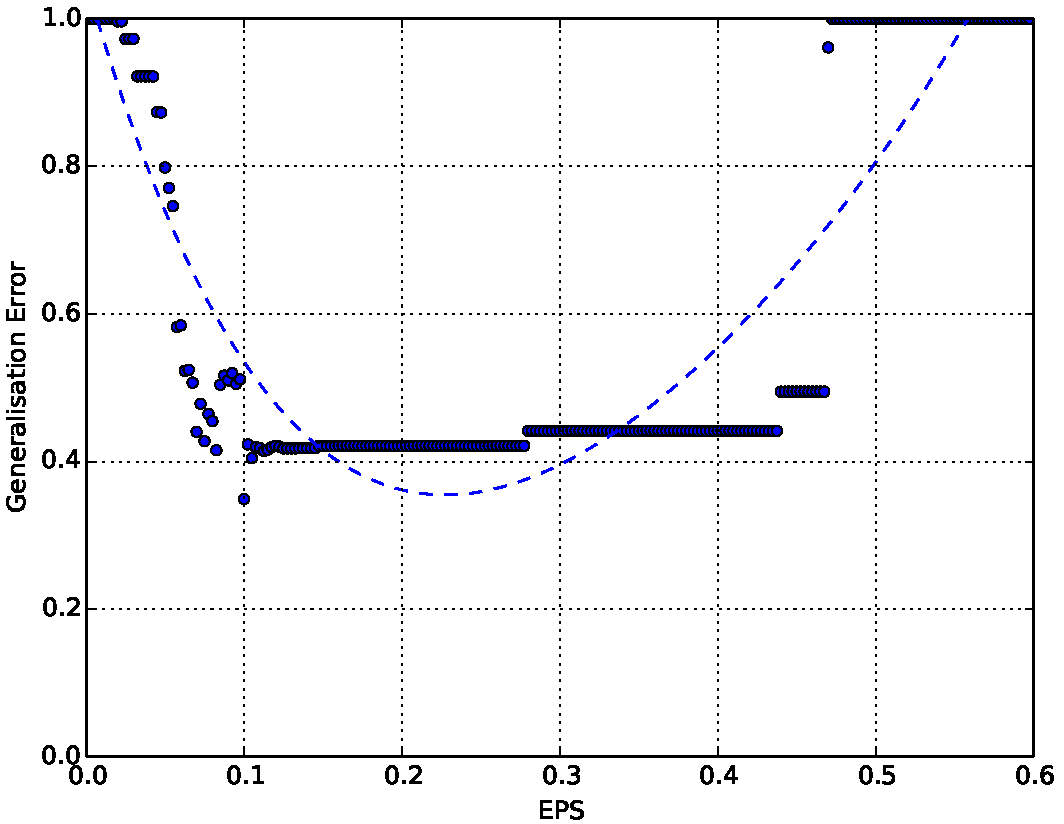
\includegraphics[height = 5cm,width = 8cm]{error.pdf}
   \caption{Generalisation error while varying the $\epsilon$ input parameter.}
   \label{fig:error}
\end{figure}




\section{Extensions}

The algorithm was revisited by its creators when they devised Generalzed-DBSCAN~\citep{ester98gdbscan}.
GDBSCAN attempts to reduce sensitivity to input parameters by comparing prospective additions to a cluster against the sparsity of the rest of the cluster. 
There's also HDBSCAN (Hierarchical) which focuses on parallel optimisation~\citep{li11}.
A subset of the original authors went on the create OPTICS (Ordering Points to Identify the Clustering Structure) which is also a density based algorithm~\citep{Ankerst99optics}.
This proved to become very popular as it performs well on datasets containing clusters of varying density.    
\cite{lian07ldbscan} developed LDBSCAN (Local-DBSCAN) which draw on both DBSCAN and OPTICS to produce an easily tunable algorithm that adapts to local cluster density.


\section{Conclusions}
DBSCAN performs well on spatial databases and can be optimised to be extremely efficient.
Datasets which are both large and spatial are common for which this algorithm is designed to classifiy.
As per most unsupervised clustering algorithms this is particularly appealing for good results whilst using simple methods. 
There are downsides to algorithm such as sensitivity to input parameters and poor performance on mixed density clustering.
As described in Section~\ref{performance} there are also cornerstone cases which can trap the density process but are easily handled by standard centroid approaches.


%TC:ignore
\bibliographystyle{ecs}
\bibliography{references}



\backmatter
\begin{appendix}

\newpage
\section{Code Listings}
\label{code}
\lstset{ %
     language=Python,                % the language of the code
  basicstyle=\footnotesize,           % the size of the fonts that are used for the code
  numbers=none,                   % where to put the line-numbers
  numberstyle=\tiny\color{black},  % the style that is used for the line-numbers
  stepnumber=2,                   % the step between two line-numbers. If it's 1, each line 
                                  % will be numbered
  numbersep=5pt,                  % how far the line-numbers are from the code
  backgroundcolor=\color{white},      % choose the background color. You must add \usepackage{color}
  showspaces=false,               % show spaces adding particular underscores
  showstringspaces=false,         % underline spaces within strings
  showtabs=false,                 % show tabs within strings adding particular underscores
  rulecolor=\color{black},        % if not set, the frame-color may be changed on line-breaks within not-black text (e.g. comments (green here))
  tabsize=2,                      % sets default tabsize to 2 spaces
  captionpos=b,                   % sets the caption-position to bottom
  breaklines=true,                % sets automatic line breaking
  breakatwhitespace=false,        % sets if automatic breaks should only happen at whitespace
  title=\lstname,                   % show the filename of files included with \lstinputlisting;
                                  % also try caption instead of title
  keywordstyle=\color{blue},          % keyword style
  commentstyle=\color{green},       % comment style
  stringstyle=\color{red},         % string literal style
  escapeinside={\%*}{*)},            % if you want to add LaTeX within your code
  morekeywords={*,...},              % if you want to add more keywords to the set
  deletekeywords={...}              % if you want to delete keywords from the given language
}

\lstinputlisting[caption=K-Means clustering.,label={KMEANS.py}]{../Code/KMEANS.py}
\newpage
\lstinputlisting[caption=WARD Clustering.,label={WARD.py}]{../Code/WARD.py}
\newpage
\lstinputlisting[caption=DBSCAN Clustering.,label={DBSCAN.py}]{../Code/DBSCAN.py}
\newpage
\lstinputlisting[caption=Tuning DBSCAN.,label={tuneDBSCAN}]{../Code/tuneDBSCAN.py}
\end{appendix}

%TC:endignore
\end{document}
%% ----------------------------------------------------------------

